\chapter{Planificación e presupostos}
\minitoc
\clearpage

Este capítulo inclúe todos os aspectos relativos á xestión do proxecto, incluíndo a planificación temporal, a metodoloxía de desenvolvemento, a xestión de riscos e as estimación dos custos ou presupostos.

\section{Xestión de riscos}

\subsection{Introdución}

O actual proxecto implica certo carácter investigador, ao ter que procurar e recopilar posíbeis fallas na emprega de contedores, unha tecnoloxía que, á súa vez, aínda ten unha vida curta no eido da supercomputación.\\

Podemos concluír pois que o nivel de incerteza do proxecto resulta bastante elevado e, polo tanto, unha boa xestión de riscos resulta crucial para o adecuado desenvolvemento do mesmo. Cómpre detectar os riscos asociados ao proxecto para evitar o incumprimento de prazos ou sobrecustos innecesarios. É esencial a identificación destes posíbeis riscos, así como a aplicación de medidas para a súa prevención, miniaturización ou eliminación. Seguiranse os seguintes pasos:

\begin{enumerate}
    \item \textbf{Identificación de riscos:} detección de ameazas que poidan pór en perigo a viabilidade e desenvolvemento do proxecto.
    
    \item \textbf{Análise e clasificación:} unha vez detectadas as ameazas existentes, serán avaliadas individualmente para determinar se supón un risco para o proxecto. Cada risco terá asociados unha probabilidade e impacto, grazas aos cales poderemos realizar unha planificación fronte a estes. De ter asociados un impacto e/ou probabilidade de suceso moi baixos, descartaranse do plan de resposta.
    
    \item \textbf{Planificación:} clasificados os riscos, serán explicadas as medidas de prevención, miniaturización ou continxencia a aplicar.
    
    \item \textbf{Seguimento:} realizados os pasos anteriores, cómpre realizar un seguimento dos riscos ao longo do proxecto para comprobar a súa evolución e posíbel materialización, co fin de dar resposta no menor tempo posíbel.
\end{enumerate}

Para comprender adecuadamente a continuación desta sección, cómpre entender unha serie de conceptos: os riscos son a probabilidade de que as ameazas actúen sobre os activos, causando danos ou perdas. Os activos son os compoñentes ou funcionalidades susceptíbeis de seren atacados, deliberada ou accidentalmente, con consecuencias para o organismo, entidade ou sistema. As vulnerabilidades son as debilidades ou falla de control que permitiría ou facilitaría que unha ameaza actúe contra un activo. Unha ameaza é unha circunstancia ou evento que pode explotar, intencionadamente ou non, unha vulnerabilidade específica. O impacto é o dano causado nun activo como resultado da explotación dunha vulnerabilidade por unha ameaza.

\subsection{Medidores dos riscos}

Os medidores dos riscos serán os seguintes:

\begin{itemize}
    \item \textbf{Probabilidade} de suceso dun risco:
    \begin{itemize}
        \item \textbf{Baixa:} menos de 25\% de posibilidades de suceso.
        \item \textbf{Media:} entre 25\% e 75\% de posibilidades de suceso.
        \item \textbf{Alta:} máis de 75\% de posibilidades de suceso.
    \end{itemize}
    
    \item \textbf{Impacto} en tempo, esforzo ou custo do suceso dun risco:
    \begin{itemize}
        \item \textbf{Insignificante:} a manifestación do risco terá unha repercusión mínima no desenvolvemento do proxecto.
        \item \textbf{Tolerábel:} a manifestación do risco provocará atrasos na realización das tarefas asociadas ao proxecto, mais será posíbel realizar a entrega do proxecto nos prazos establecidos.
        \item \textbf{Serio:} a manifestación do risco provocará que a entrega do TFG se realice noutra convocatoria.
        \item \textbf{Catastrófico:} a manifestación do risco provocará que non sexa posíbel realizar a entrega do proxecto no prazo dun ano. Tal feito implicaría refacer o TFG enteiramente.
    \end{itemize}
    
    \item \textbf{Nivel de exposición:} combinación dos anteriores valores de probabilidade e impacto, converténdoos nunha medida tanxíbel. Para isto é preciso asociar os anteriores medidores con valores numéricos. A valoración da probabilidade pode ser consultada na táboa \ref{valoracionProbabilidade} e valoración do impacto, na táboa \ref{valoracionImpacto}.
    
\begin{table}[]
\centering
\caption{Valoración da probabilidade}
\label{valoracionProbabilidade}
\begin{tabular}{|c|c|}
\hline
\textbf{Probabilidade} & \textbf{Valor numérico asociado} \\ \hline
Baixa & 0.2 \\ \hline
Media & 0.5 \\ \hline
Alta & 0.8 \\ \hline
\end{tabular}
\end{table}

\begin{table}[]
\centering
\caption{Valoración do impacto}
\label{valoracionImpacto}
\begin{tabular}{|c|c|}
\hline
\textbf{Impacto} & \textbf{Valor numérico asociado} \\ \hline
Insignificante & 0.1 \\ \hline
Tolerábel & 0.4 \\ \hline
Serio & 0.6 \\ \hline
Catastrófico & 0.9 \\ \hline
\end{tabular}
\end{table}

Establecidas estas valoracións, é posíbel obter o nivel de exposición, resultado do produto dos dous valores anteriormente definidos, reflectido na táboa \ref{nivelExposicionRisco}. Serán definidos os seguintes tipos de exposición segundo os valores obtidos en dita táboa:

\begin{itemize}
    \item \textbf{Baixa:} valor da exposición comprendido entre 0 e 0.15.
    \item \textbf{Media:} valor da exposición comprendido entre 0.16 e 0.4.
    \item \textbf{Alta:} valor da exposición estritamente maior que 0.4.
\end{itemize}


\begin{table}[]
\centering
\caption{Nivel de exposición ao risco}
\label{nivelExposicionRisco}
\resizebox{\textwidth}{!}{%
\begin{tabular}{|c|c|c|c|c|c|}
\hline
\multicolumn{2}{|c|}{\multirow{2}{*}{}} & \multicolumn{4}{c|}{Impacto} \\ \cline{3-6} 
\multicolumn{2}{|c|}{} & Insignificante (0.1) & Tolerábel (0.4) & Serio (0.6) & Catastrófico (0.9) \\ \hline
\multirow{3}{*}{Probabilidade} & Baixa (0.2) & 0.02 & 0.08 & 0.12 & 0.18 \\ \cline{2-6} 
 & Media (0.5) & 0.05 & 0.2 & 0.3 & 0.45 \\ \cline{2-6} 
 & Alta (0.8) & 0.08 & 0.32 & 0.48 & 0.72 \\ \hline
\end{tabular}
}
\end{table}

\end{itemize}

\subsection{Tipos de riscos}

Para a clasificación dos riscos seguirase a categorización de Sommerville \cite{Sommerville}, segundo a cal existen tres tipos de riscos:

\begin{enumerate}
    \item \textbf{De proxecto:} afectan á programación temporal ou aos recursos.
    \item \textbf{De produto:} afectan á calidade ou desempeño do produto.
    \item \textbf{De negocio:} afectan á organización responsábel do desenvolvemento.
\end{enumerate}

\subsection{Tipos de estratexias a seguir}

Unha vez identificados os posíbeis riscos que poidan afectar ao proxecto, cómpre realizar unha análise de cada un deles, para poder realizar a súa categorización en base á súa relevancia. Contémplanse varios métodos para combater un risco potencial:

\begin{itemize}
    \item \textbf{Prevención:} baséase en reducir a probabilidade de que un risco se materialice.
    \item \textbf{Miniaturización:} baséase en reducir o impacto xerado polo risco.
    \item \textbf{Aceptación:} baséase en asumir o impacto asociado ao risco e as súas consecuencias.
    \item \textbf{Continxencia:} baséase na aplicación dun plan de continxencia no que aparezan accións a realizar en caso de que aconteza un risco.
    \item \textbf{Transferencia:} baséase no traspaso do risco a outra entidade que o xestione por nós.
\end{itemize}

\subsection{Identificación de ameazas}

\begin{table}[H]
\caption{Ameaza A1}
\label{A1}
\begin{tabularx}{\textwidth}{|l|X|}
\hline
\textbf{Identificador} & A1 \\ \hline
\textbf{Nome} & Perda do repositorio local. \\ \hline
\textbf{Descrición} & O repositorio gardado no equipo de traballo pérdese por mor dun fallo no disco duro. Isto provoca que se perda a última versión dos elementos da configuración. \\ \hline
\end{tabularx}
\end{table}

\begin{table}[H]
\caption{Ameaza A2}
\label{A2}
\begin{tabularx}{\textwidth}{|l|X|}
\hline
\textbf{Identificador} & A2 \\ \hline
\textbf{Nome} & Atraso na realización dun fito. \\ \hline
\textbf{Descrición} & Un fito reflectido na planificación inicial do proxecto, é dicir, no anteproxecto, non é acadado no prazo previsto debido a improvisos na realización do traballo. \\ \hline
\end{tabularx}
\end{table}

\begin{table}[H]
\caption{Ameaza A3}
\label{A3}
\begin{tabularx}{\textwidth}{|l|X|}
\hline
\textbf{Identificador} & A3 \\ \hline
\textbf{Nome} & Elementos da configuración non identificados. \\ \hline
\textbf{Descrición} & Son ignorados algúns elementos da configuración á hora de realizar a identificación dos mesmos, polo que non serán xestionados no proceso de xestión da configuración a empregar no proxecto. \\ \hline
\end{tabularx}
\end{table}

\begin{table}[H]
\caption{Ameaza A4}
\label{A4}
\begin{tabularx}{\textwidth}{|l|X|}
\hline
\textbf{Identificador} & A4 \\ \hline
\textbf{Nome} & Identificación de elementos da configuración innecesarios. \\ \hline
\textbf{Descrición} & Son detectados elementos da configuración que deben ser xestionados, mais que finalmente non resultan relevantes para a execución do proxecto, o que provoca atrasos á hora de realizar a xestión da configuración do proxecto. \\ \hline
\end{tabularx}
\end{table}

\begin{table}[H]
\caption{Ameaza A5}
\label{A5}
\begin{tabularx}{\textwidth}{|l|X|}
\hline
\textbf{Identificador} & A5 \\ \hline
\textbf{Nome} & Definición dun proceso da xestión da configuración ineficaz e/ou incorrecto. \\ \hline
\textbf{Descrición} & Á hora de executar o proceso de configuración, obsérvanse erros que dificultan a consecución dos obxectivos precisos para a realización do proxecto. \\ \hline
\end{tabularx}
\end{table}

\begin{table}[H]
\caption{Ameaza A6}
\label{A6}
\begin{tabularx}{\textwidth}{|l|X|}
\hline
\textbf{Identificador} & A6 \\ \hline
\textbf{Nome} & Non é definido un proceso de xestión da configuración. \\ \hline
\textbf{Descrición} & Non é definido un proceso de xestión da configuración na fase inicial do proxecto. \\ \hline
\end{tabularx}
\end{table}

\begin{table}[H]
\caption{Ameaza A7}
\label{A7}
\begin{tabularx}{\textwidth}{|l|X|}
\hline
\textbf{Identificador} & A7 \\ \hline
\textbf{Nome} & Proceso de xestión da configuración excesivamente burocrático. \\ \hline
\textbf{Descrición} & O proceso de xestión da configuración elixido ou deseñado require dunha cantidade de documentación moi superior á precisa. Isto podería chegar a provocar atrasos nos fitos do proxecto, pois é destinada unha cantidade de tempo significativa no tratamento destes documentos. \\ \hline
\end{tabularx}
\end{table}

\begin{table}[H]
\caption{Ameaza A8}
\label{A8}
\begin{tabularx}{\textwidth}{|l|X|}
\hline
\textbf{Identificador} & A8 \\ \hline
\textbf{Nome} & Ausencia de copia de seguridade do repositorio. \\ \hline
\textbf{Descrición} & O repositorio do proxecto está almacenado nunha única localización e dita localización perde os datos correspondentes ao proxecto. \\ \hline
\end{tabularx}
\end{table}

\begin{table}[H]
\caption{Ameaza A9}
\label{A9}
\begin{tabularx}{\textwidth}{|l|X|}
\hline
\textbf{Identificador} & A9 \\ \hline
\textbf{Nome} & Entrega dunha versión incorrecta. \\ \hline
\textbf{Descrición} & Á hora de realizar a entrega final prodúcese unha confusión na versión a entregar, o que provoca que se entregue unha versión anterior á final. \\ \hline
\end{tabularx}
\end{table}

\begin{table}[H]
\caption{Ameaza A10}
\label{A10}
\begin{tabularx}{\textwidth}{|l|X|}
\hline
\textbf{Identificador} & A10 \\ \hline
\textbf{Nome} & Incumprimento das horas de traballo. \\ \hline
\textbf{Descrición} & O proxecto débese axustar a unhas horas establecidas, correspondentes ao número de créditos asinados á materia do Traballo de Fin de Grao. No caso de incumprir a estimación temporal debe ser exposta unha razón. \\ \hline
\end{tabularx}
\end{table}

\begin{table}[H]
\caption{Ameaza A11}
\label{A11}
\begin{tabularx}{\textwidth}{|l|X|}
\hline
\textbf{Identificador} & A11 \\ \hline
\textbf{Nome} & Actualizacións do repositorio demasiado espazadas no tempo.  \\ \hline
\textbf{Descrición} & O tempo entre as diferentes actualizacións no repositorio é excesivamente longo, o que pode provocar que de querer volver a unha versión antiga, pérdanse cambios que poidan ser considerados de relevancia. \\ \hline
\end{tabularx}
\end{table}

\begin{table}[H]
\caption{Ameaza A12}
\label{A12}
\begin{tabularx}{\textwidth}{|l|X|}
\hline
\textbf{Identificador} & A12 \\ \hline
\textbf{Nome} & Equipo de traballo avariado. \\ \hline
\textbf{Descrición} & O equipo de traballo co que conta o estudante fica avariado, impedindo a realización do proxecto. \\ \hline
\end{tabularx}
\end{table}

\begin{table}[H]
\caption{Ameaza A13}
\label{A13}
\begin{tabularx}{\textwidth}{|l|X|}
\hline
\textbf{Identificador} & A13 \\ \hline
\textbf{Nome} & Roubo de material \\ \hline
\textbf{Descrición} & Perda de material (non dixital) por mor dun roubo no lugar de traballo. \\ \hline
\end{tabularx}
\end{table}

\begin{table}[H]
\caption{Ameaza A14}
\label{A14}
\begin{tabularx}{\textwidth}{|l|X|}
\hline
\textbf{Identificador} & A14 \\ \hline
\textbf{Nome} & Caída dun dos portais de contedores a empregar. \\ \hline
\textbf{Descrición} & Un dos portais de onde se descargan as imaxes dos contedores a empregar para o desenvolvemento do proxecto cae, quedando inoperante e impedindo a obtención de imaxes importantes para o traballo. \\ \hline
\end{tabularx}
\end{table}

\begin{table}[H]
\caption{Ameaza A15}
\label{A15}
\begin{tabularx}{\textwidth}{|l|X|}
\hline
\textbf{Identificador} & A15 \\ \hline
\textbf{Nome} & Caída dos entornos de pre-produción ou produción. \\ \hline
\textbf{Descrición} & Os entornos de pre-predución (computación na nube) ou produción do \gls{CESGA} caen, impedindo a realización das probas precisas para o desenvolvemento dou proxecto, ou ocasionando a perda de información importante. \\ \hline
\end{tabularx}
\end{table}

\subsection{Identificación de activos}

\begin{enumerate}[{ACT}1: ]
    \item Equipo de traballo.
    \item Memoria do proxecto.
    \item Repositorio.
    \item Proceso de xestión da configuración.
    \item Contedores sobre os que realizar as probas.
    \item Material de traballo non dixital: apuntamentos, libros, etc.
    \item Infraestrutura do \gls{CESGA}.
    \item Imaxes e diagramas.
    \item \textit{Scripts}.
\end{enumerate}

\subsection{Análise de riscos}

Como xa foi visto, os riscos son a probabilidade de que as ameazas actúen sobre os activos, causando danos ou perdas, polo que cada risco estará relacionado cunha das ameazas estudadas previamente. Está correlación virá indicada polo seu número do identificador, que será o mesmo para a ameaza e o risco.

\begin{table}[H]
\centering
\caption{Risco R1}
\label{R1}
\begin{tabularx}{\textwidth}{|l|l|l|l|}
\hline
\textbf{Identificador} & R1 & \textbf{Tipo de risco} & De produto \\ \hline
\textbf{Probabilidade} & Baixa & \textbf{Impacto} & Tolerábel \\ \hline
\textbf{Exposición} & Baixa & \textbf{Activos afectados} & ACT1, ACT2, ACT8, ACT9 \\ \hline
\multicolumn{1}{|l|}{\textbf{Tratamento}} & \multicolumn{3}{X|}{\tabitem \textbf{Aceptación:} enténdese que os últimos datos xa están perdidos, ao non ter realizado unha actualización do repositorio remoto. Ao ter unha exposición baixa podemos aceptar este risco sen moito problema, soamente habería que repetir os últimos avances.} \\ \hline
\multicolumn{1}{|l|}{\textbf{Indicadores}} & \multicolumn{3}{X|}{O sistema non permite acceder aos últimos cambios realizados en disco no proxecto.} \\ \hline
\end{tabularx}
\end{table}

\begin{table}[H]
\centering
\caption{Risco R2}
\label{R3}
\begin{tabularx}{\textwidth}{|l|l|l|l|}
\hline
\textbf{Identificador} & R2 & \textbf{Tipo de risco} & De proxecto \\ \hline
\textbf{Probabilidade} & Media & \textbf{Impacto} & Tolerábel \\ \hline
\textbf{Exposición} & Media & \textbf{Activos afectados} & ACT2 \\ \hline
\multicolumn{1}{|l|}{\textbf{Tratamento}} & \multicolumn{3}{X|}{\tabitem \textbf{Prevención:} realización dunha boa planificación.


\tabitem \textbf{Miniaturización:} incluír tarefas con pouca relevancia nunha sección de tarefas excluídas.} \\ \hline
\multicolumn{1}{|l|}{\textbf{Indicadores}} & \multicolumn{3}{X|}{Algunha das tarefas a realizar, definidas no anteproxecto, superou por un prazo superior a 2 días o seu tempo previsto de execución.} \\ \hline
\end{tabularx}
\end{table}

\begin{table}[H]
\centering
\caption{Risco R3}
\label{R3}
\begin{tabularx}{\textwidth}{|l|l|l|l|}
\hline
\textbf{Identificador} & R3 & \textbf{Tipo de risco} & De produto \\ \hline
\textbf{Probabilidade} & Media & \textbf{Impacto} & Tolerábel \\ \hline
\textbf{Exposición} & Media & \textbf{Activos afectados} & ACT3, ACT4 \\ \hline
\multicolumn{1}{|l|}{\textbf{Tratamento}} & \multicolumn{3}{X|}{\tabitem \textbf{Prevención:} identificación adecuada dos elementos da configuración e realización dunha xestión da configuración simple e eficiente.


\tabitem \textbf{Miniaturización:} detectado o problema, realizar modificacións na xestión da configuración para incluír o novo elemento non identificado previamente. Posto que o equipo de traballo é dunha soa persoa, non debería haber problema por realizar cambios pequenos e xustificados na xestión da configuración.} \\ \hline
\multicolumn{1}{|l|}{\textbf{Indicadores}} & \multicolumn{3}{X|}{Cando o proxecto avanza, obsérvase que hai elementos que non están sendo contemplados na xestión da configuración, ao non ter sido considerados elementos da configuración en si.} \\ \hline
\end{tabularx}
\end{table}

\begin{table}[H]
\centering
\caption{Risco R4}
\label{R4}
\begin{tabularx}{\textwidth}{|l|l|l|l|}
\hline
\textbf{Identificador} & R4 & \textbf{Tipo de risco} & De produto \\ \hline
\textbf{Probabilidade} & Media & \textbf{Impacto} & Tolerábel \\ \hline
\textbf{Exposición} & Media & \textbf{Activos afectados} & ACT3, ACT4 \\ \hline
\multicolumn{1}{|l|}{\textbf{Tratamento}} & \multicolumn{3}{X|}{\tabitem \textbf{Prevención:} identificación adecuada dos elementos da configuración e realización dunha xestión da configuración simple e eficiente.


\tabitem \textbf{Miniaturización:} detectado o problema, realizar modificacións na xestión da configuración para excluír os elementos sobrantes. Posto que o equipo de traballo é dunha soa persoa, non debería haber problema por realizar cambios pequenos e xustificados na xestión da configuración.} \\ \hline
\multicolumn{1}{|l|}{\textbf{Indicadores}} & \multicolumn{3}{X|}{Cando o proxecto avanza, obsérvase que hai elementos que non son precisos para o correcto desenvolvemento do proxecto, polo que o seu control implica unha perda de tempo innecesaria.} \\ \hline
\end{tabularx}
\end{table}


\begin{table}[H]
\centering
\caption{Risco R5}
\label{R5}
\begin{tabularx}{\textwidth}{|l|l|l|l|}
\hline
\textbf{Identificador} & R5 & \textbf{Tipo de risco} & De produto \\ \hline
\textbf{Probabilidade} & Media & \textbf{Impacto} & Tolerábel \\ \hline
\textbf{Exposición} & Media & \textbf{Activos afectados} & ACT3, ACT4 \\ \hline
\multicolumn{1}{|l|}{\textbf{Tratamento}} & \multicolumn{3}{X|}{\tabitem \textbf{Prevención:} deseño dunha xestión da configuración adecuada ao proxecto e que resulte eficaz e eficiente.


\tabitem \textbf{Miniaturización:} detectado o problema, realizar modificacións na xestión da configuración para que esta se adapte correctamente ao proxecto. Posto que o equipo de traballo é dunha soa persoa, non debería haber problema por realizar cambios pequenos e xustificados na xestión da configuración.} \\ \hline
\multicolumn{1}{|l|}{\textbf{Indicadores}} & \multicolumn{3}{X|}{Cando o proxecto avanza, obsérvanse serios problemas para levar a cabo a xestión da configuración (por exemplo, modelos inservíbeis ou incompletos).} \\ \hline
\end{tabularx}
\end{table}


\begin{table}[H]
\centering
\caption{Risco R6}
\label{R6}
\begin{tabularx}{\textwidth}{|l|l|l|l|}
\hline
\textbf{Identificador} & R6 & \textbf{Tipo de risco} & De produto \\ \hline
\textbf{Probabilidade} & Baixa & \textbf{Impacto} & Serio \\ \hline
\textbf{Exposición} & Baixa & \textbf{Activos afectados} & ACT3, ACT4 \\ \hline
\multicolumn{1}{|l|}{\textbf{Tratamento}} & \multicolumn{3}{X|}{\tabitem \textbf{Prevención:} deseño dunha xestión da configuración adecuada ao inicio do proxecto.} \\ \hline
\multicolumn{1}{|l|}{\textbf{Indicadores}} & \multicolumn{3}{X|}{Non é posíbel realizar unha xestión da configuración e non están quedando almacenados os diferentes cambios no proxecto en ningún momento.} \\ \hline
\end{tabularx}
\end{table}


\begin{table}[H]
\centering
\caption{Risco R7}
\label{R7}
\begin{tabularx}{\textwidth}{|l|l|l|l|}
\hline
\textbf{Identificador} & R7 & \textbf{Tipo de risco} & De produto \\ \hline
\textbf{Probabilidade} & Media & \textbf{Impacto} & Tolerábel \\ \hline
\textbf{Exposición} & Media & \textbf{Activos afectados} & ACT3, ACT4 \\ \hline
\multicolumn{1}{|l|}{\textbf{Tratamento}} & \multicolumn{3}{X|}{\tabitem \textbf{Prevención:} deseño dunha xestión da configuración adecuada ao proxecto e que resulte eficaz e eficiente.


\tabitem \textbf{Miniaturización:} detectado o problema, realizar modificacións na xestión da configuración para que esta se adapte correctamente ao proxecto. Posto que o equipo de traballo é dunha soa persoa, non debería haber problema por realizar cambios pequenos e xustificados na xestión da configuración.} \\ \hline
\multicolumn{1}{|l|}{\textbf{Indicadores}} & \multicolumn{3}{X|}{Cando o proxecto avanza, detéctase unha perda de tempo excesiva no tratamento da xestión da configuración.} \\ \hline
\end{tabularx}
\end{table}


\begin{table}[H]
\centering
\caption{Risco R8}
\label{R8}
\begin{tabularx}{\textwidth}{|l|l|l|l|}
\hline
\textbf{Identificador} & R8 & \textbf{Tipo de risco} & De proxecto \\ \hline
\textbf{Probabilidade} & Baixa & \textbf{Impacto} & Catastrófico \\ \hline
\textbf{Exposición} & Media & \textbf{Activos afectados} & ACT2, ACT3, ACT8, ACT9 \\ \hline
\multicolumn{1}{|l|}{\textbf{Tratamento}} & \multicolumn{3}{X|}{\tabitem \textbf{Prevención:} establecer o proceso de xestión da configuración de tal forma que o repositorio de traballo estea almacenado en múltiples localizacións, preferibelmente afastadas no espazo.} \\ \hline
\multicolumn{1}{|l|}{\textbf{Indicadores}} & \multicolumn{3}{X|}{Soamente existe unha copia do proxecto, non sendo posíbel acceder a outras copias de seguridade.} \\ \hline
\end{tabularx}
\end{table}

\begin{table}[H]
\centering
\caption{Risco R9}
\label{R9}
\begin{tabularx}{\textwidth}{|l|l|l|l|}
\hline
\textbf{Identificador} & R9 & \textbf{Tipo de risco} & De produto \\ \hline
\textbf{Probabilidade} & Baixa & \textbf{Impacto} & Serio \\ \hline
\textbf{Exposición} & Baixa & \textbf{Activos afectados} & ACT2, ACT8, ACT9 \\ \hline
\multicolumn{1}{|l|}{\textbf{Tratamento}} & \multicolumn{3}{X|}{\tabitem \textbf{Prevención:} revisión ao menos dúas veces de que a versión a entregar concorda coas últimas modificacións realizadas no proxecto.} \\ \hline
\multicolumn{1}{|l|}{\textbf{Indicadores}} & \multicolumn{3}{X|}{O proxecto obtido pola comisión de traballos de fin de grao non é o mesmo que a última versión que posúe o autor.} \\ \hline
\end{tabularx}
\end{table}

\begin{table}[H]
\centering
\caption{Risco R10}
\label{R10}
\begin{tabularx}{\textwidth}{|l|l|l|l|}
\hline
\textbf{Identificador} & R10 & \textbf{Tipo de risco} & De proxecto \\ \hline
\textbf{Probabilidade} & Alta & \textbf{Impacto} & Serio \\ \hline
\textbf{Exposición} & Alta & \textbf{Activos afectados} & ACT2 \\ \hline
\multicolumn{1}{|l|}{\textbf{Tratamento}} & \multicolumn{3}{X|}{\tabitem \textbf{Prevención:} realización dunha boa planificación temporal e seguimento dunha metodoloxía áxil para evitar os riscos asociados á incerteza do proxecto.} \\ \hline
\multicolumn{1}{|l|}{\textbf{Indicadores}} & \multicolumn{3}{X|}{\tabitem As tarefas definidas no anteproxecto están levando máis tempo do esperado.

\tabitem Non se está seguindo ningunha metodoloxía de traballo áxil.} \\ \hline
\end{tabularx}
\end{table}

\begin{table}[H]
\centering
\caption{Risco R11}
\label{R11}
\begin{tabularx}{\textwidth}{|l|l|l|l|}
\hline
\textbf{Identificador} & R11 & \textbf{Tipo de risco} & De proxecto \\ \hline
\textbf{Probabilidade} & Media & \textbf{Impacto} & Tolerábel \\ \hline
\textbf{Exposición} & Media & \textbf{Activos afectados} & \scriptsize{ACT2, ACT3, ACT4, ACT8, ACT9} \\ \hline
\multicolumn{1}{|l|}{\textbf{Tratamento}} & \multicolumn{3}{X|}{\tabitem \textbf{Prevención:} establecer na xestión da configuración un procedemento de xestión de cambios en intres reducidos de tempo.} \\ \hline
\multicolumn{1}{|l|}{\textbf{Indicadores}} & \multicolumn{3}{X|}{Cando se quere retroceder a unha versión anterior empregando a xestión da configuración, moitos datos son perdidos, que ben poderían estar diferenciados en \textit{commits} distintos para evitar a súa perda.} \\ \hline
\end{tabularx}
\end{table}

\begin{table}[H]
\centering
\caption{Risco R12}
\label{R12}
\begin{tabularx}{\textwidth}{|l|l|l|l|}
\hline
\textbf{Identificador} & R12 & \textbf{Tipo de risco} & De negocio \\ \hline
\textbf{Probabilidade} & Baixa & \textbf{Impacto} & Catastrófico \\ \hline
\textbf{Exposición} & Media & \textbf{Activos afectados} & ACT1 \\ \hline
\multicolumn{1}{|l|}{\textbf{Tratamento}} & \multicolumn{3}{X|}{\tabitem \textbf{Prevención:} poder contar cun equipo de reposto para poder continuar co traballo nun período inferior a 12 horas.} \\ \hline
\multicolumn{1}{|l|}{\textbf{Indicadores}} & \multicolumn{3}{X|}{Non é posíbel traballar co equipo de traballo ou facelo de xeito adecuado para o desenvolvemento do proxecto.} \\ \hline
\end{tabularx}
\end{table}

\begin{table}[H]
\centering
\caption{Risco R13}
\label{R13}
\begin{tabularx}{\textwidth}{|l|l|l|l|}
\hline
\textbf{Identificador} & R13 & \textbf{Tipo de risco} & De negocio \\ \hline
\textbf{Probabilidade} & Baixa & \textbf{Impacto} & Serio \\ \hline
\textbf{Exposición} & Baixa & \textbf{Activos afectados} & ACT1, ACT6, ACT7 \\ \hline
\multicolumn{1}{|l|}{\textbf{Tratamento}} & \multicolumn{3}{X|}{\tabitem \textbf{Transferencia:} o \gls{CESGA} dispón de medidas físicas de seguridade para evitar este tipo de sucesos. A zona de traballo non é accesíbel sen previa identificación e existe seguridade mediante gravación do centro.} \\ \hline
\multicolumn{1}{|l|}{\textbf{Indicadores}} & \multicolumn{3}{X|}{Desaparece parte ou a totalidade dos materiais físicos de traballo.} \\ \hline
\end{tabularx}
\end{table}

\begin{table}[H]
\centering
\caption{Risco R14}
\label{R14}
\begin{tabularx}{\textwidth}{|l|l|l|l|}
\hline
\textbf{Identificador} & R14 & \textbf{Tipo de risco} & De proxecto \\ \hline
\textbf{Probabilidade} & Baixa & \textbf{Impacto} & Serio \\ \hline
\textbf{Exposición} & Baixa & \textbf{Activos afectados} & ACT5 \\ \hline
\multicolumn{1}{|l|}{\textbf{Tratamento}} & \multicolumn{3}{X|}{\tabitem \textbf{Aceptación:} posto que se trata dun servizo completamente externo, non é posíbel aplicar moitas medidas. Tentarase traballar coas imaxes xa almacenadas no equipo local, mais no caso de querer facer probas directamente co portal non haberá nada que facer, agás agardar á súa recuperación.} \\ \hline
\multicolumn{1}{|l|}{\textbf{Indicadores}} & \multicolumn{3}{X|}{Resulta imposíbel acceder a algún dos portais de imaxes de contedores cos que se traballa ao longo do proxecto (obtención de erro 404 ou similar).} \\ \hline
\end{tabularx}
\end{table}

\begin{table}[H]
\centering
\caption{Risco R15}
\label{R15}
\begin{tabularx}{\textwidth}{|l|l|l|l|}
\hline
\textbf{Identificador} & R15 & \textbf{Tipo de risco} & De negocio \\ \hline
\textbf{Probabilidade} & Baixa & \textbf{Impacto} & Catastrófico \\ \hline
\textbf{Exposición} & Media & \textbf{Activos afectados} & ACT7 \\ \hline
\multicolumn{1}{|l|}{\textbf{Tratamento}} & \multicolumn{3}{X|}{\tabitem \textbf{Transferencia:} o \gls{CESGA} dispón de medidas para minimizar o impacto en caso de que este tipo de risco se materialice. Por exemplo, existen copias de seguridade programadas para evitar a perda da totalidade do traballo. Tamén existen medidas de prevención como un xerador de electricidade ou unha múltiple conexión coa rede externa mediante diversos servizos para asegurar o continuo funcionamento do sistema.} \\ \hline
\multicolumn{1}{|l|}{\textbf{Indicadores}} & \multicolumn{3}{X|}{Resulta imposíbel acceder aos entornos de pre-produción ou produción.} \\ \hline
\end{tabularx}
\end{table}

\subsection{Seguimento dos riscos}

Realizados os pasos de identificación, análise, clasificación e planificación, só queda realizar un seguimento dos riscos ao longo da vida do proxecto. Este seguimento seguiuse rigorosamente, feito que permitiu a detección da materialización dun dos riscos identificados.

\subsubsection{Seguimento do risco R14}

Materializouse o risco R14, a caída dun dos portais de imaxes de contedores, o Docker Hub. As medidas a tomar neste caso eran simplemente de aceptación, ao non ter control sobre servizos externos. Afortunadamente, este risco materializouse o 24 de xuño do 2018, cando todas as probas relacionadas con este portal xa estaban satisfactoriamente completadas. De todos os xeitos, a caída foi solucionada axiña polos responsábeis do portal, polo que non tería moito impacto no desenvolvemento do proxecto de ter ocorrido noutro momento no que si fixera falla a emprega deste portal (simplemente a agarda dunhas horas).\\

A figura \ref{caidaAgora} amosa a caída ou falla dalgúns dos sistemas do Docker Hub o día 24 de xuño de 2018, grazas a ferramenta de seguimento que Docker dispón ao público, o \textit{Docker System Status}\footnote{\url{https://status.docker.com/}}. A figura \ref{caidaPasada} amosa os problemas presentados no sistema dende unha ollada histórica, superado xa o incidente.\\

\begin{figure}
\centerline{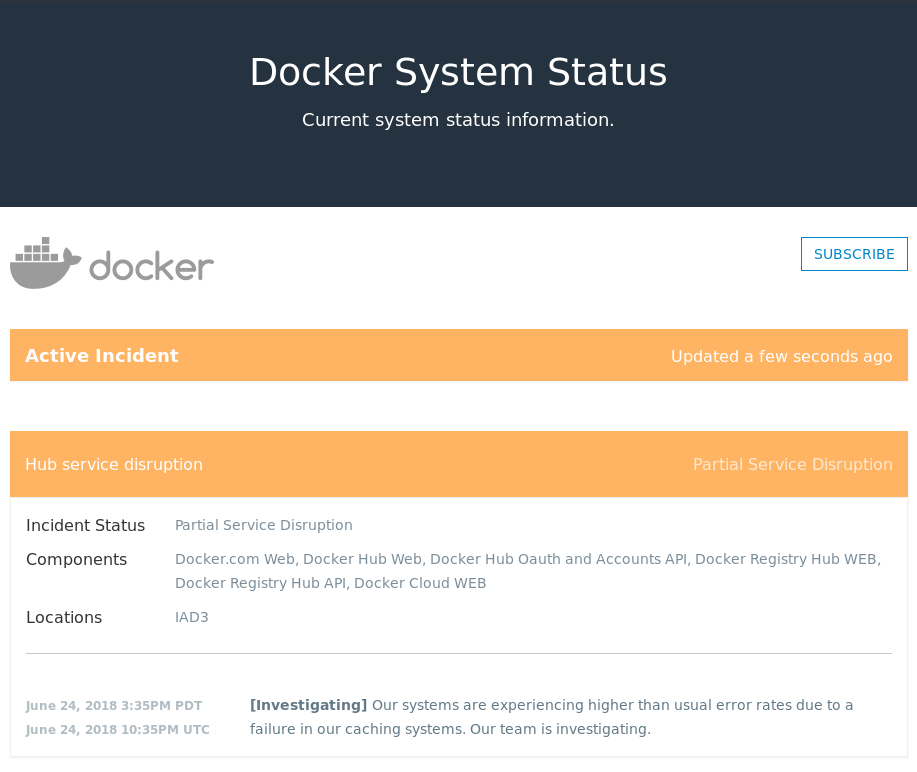
\includegraphics[width=15cm]{figuras/caidaAgora.png}}
\caption{Caída dos sistemas do Docker Hub}
\label{caidaAgora}
\end{figure}

\begin{figure}
\centerline{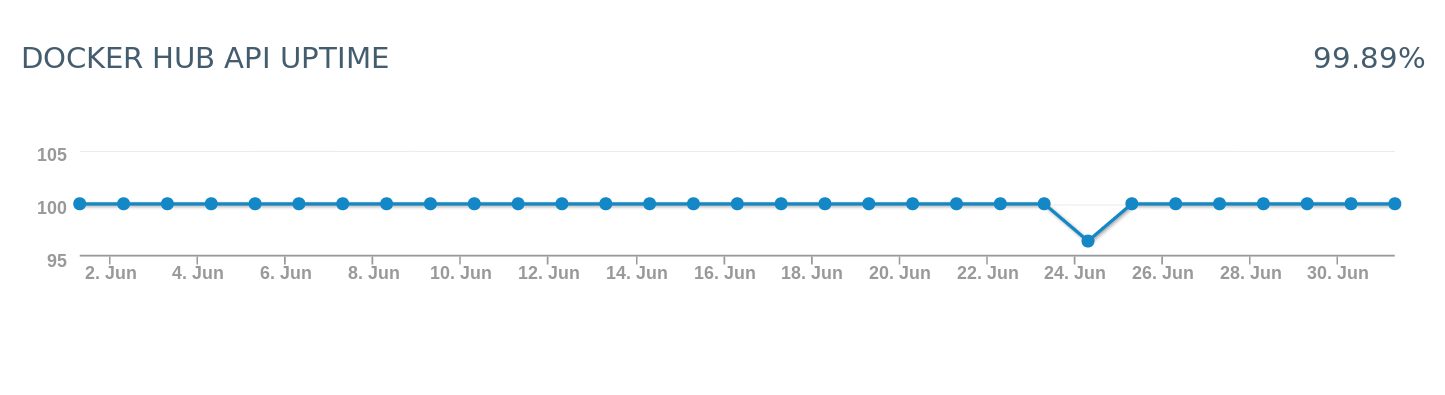
\includegraphics[width=15cm]{figuras/caidaPasada.png}}
\caption{Histórico do estado de saúde dos sistemas do Docker Hub}
\label{caidaPasada}
\end{figure}

O indicador presentado para a detección da materialización deste risco foi a obtención de erros ao tentar obter imaxes do servizo.

\begin{lstlisting}[,caption={Erro 503 ao tentar traballar co Docker Hub}]
Error response from daemon: get https://registry-1.docker.io/v2/library/...: received unexpected HTTP status: 503 Service Unavailable.
\end{lstlisting}

\section{Xestión da configuración}

\subsection{Identificación dos elementos da configuración}

Enténdese por elemento da configuración cada un dos elementos do proxecto que se vexan afectados pola xestión da configuración. Os elementos identificados son:

\begin{itemize}
    \item \textbf{Memoria do proxecto:} a presente memoria do proxecto. Inclúe os resultados do estudo, as recomendacións de prácticas a aplicar e unha serie de conclusións e traballo futuro.
    \item \textbf{Código fonte dos diferentes \textit{scripts} empregados:} código fonte cos diferentes comandos a aplicar para a realización das probas indicadas ao longo do proxecto.
    \item \textbf{Diagramas e figuras realizadas:} diagramas elaborados coa ferramenta en liña Draw.io\footnote{\url{https://www.draw.io/}} para a explicación visual de certos aspectos do proxecto. Inclúe tamén a súa representación en \gls{XML} para a posíbel aplicación de futuras modificacións.
\end{itemize}

As imaxes modificadas dos contedores de probas quedaron descartados na xestión da configuración, posto que se entende que non son realizadas configuracións complexas. Así, basta con aplicar os \textit{scripts} sobre imaxes xestionadas por terceiros e dun xeito sinxelo e rápido será posíbel acadar a reproducibilidade das probas.

\subsection{Control de cambios}

A xestión da configuración limitarase ao control de versións dos diferentes elementos da configuración. Tamén cabe indicar que dito control de cambios será levado a cabo soamente por unha persoa, o autor do proxecto. 

\subsection{Control de versións}

Para a realización do control de versión dos elementos da configuración empregarase a plataforma GitHub\footnote{\url{https://github.com/}}, cuxo principal servizo é a emprega de Git, un sistema de control de versións que traza os cambios en ficheiros, de forma remota. Nesta plataforma creouse un repositorio privado no que o único editor de contido existente no proxecto traballa sobre a rama ``\textit{master}'' do mesmo. Indicar que, aínda que se detectaron diferentes elementos da configuración, todos levarán a súa xestión de cambios baixo o mesmo repositorio e de forma conxunta. No referente á súa utilización, cada cambio é acompañado por unha mensaxe explicativa do mesmo e estes cambios non teñen por que estar necesariamente asociados á finalización dunha tarefa, senón que calquera avance considerado de relevancia é gardado para evitar os riscos relacionados coa perda da información no equipo local. A xestión da configuración resulta moi lixeira ao ser soamente unha persoa a que realiza todos os cambios.\\

A memoria, ao ser desenvolvida na plataforma en liña de edición de textos \LaTeX, Sharelatex\footnote{\url{https://www.sharelatex.com/}}, tamén podería dispor dun sistema adicional e independente de control de versións. Non obstante, este é un sistema \textit{premium} da plataforma, cuns custos asociados, do que non se disporá. Enténdese que co control de versións sobre a anteriormente nomeada plataforma GitHub é suficiente.\\

Finalmente, para facilitar as tarefas de sincronización co repositorio remoto de GitHub, farase emprega do software GitKraken\footnote{\url{https://www.gitkraken.com/}}, unha interface visual multiplataforma para Git.

\section{Planificación temporal}

\subsection{Metodoloxía de traballo}

\subsubsection{Diferenciación xeral das metodoloxías de traballo}

O primeiro paso a realizar antes de poder realizar unha adecuada planificación temporal é o de escoller unha metodoloxía de traballo. É imprescindíbel tomar esta decisión dun xeito adecuado, posto que unha elección errónea podería levar ao incumprimento de entregas en data ou, no peor dos casos, á cancelación da totalidade do proxecto. No entanto, cómpre comprendermos que non existe unha metodoloxía adecuada para todos os tipos de proxecto, senón que certas metodoloxías se adaptan mellor a certos escenarios de traballo. Para realizar esta elección, dividiremos primeiramente as metodoloxías en dous grandes bloques:

\begin{itemize}
    \item \textbf{Metodoloxías clásicas:} están baseadas nunha planificación temporal definida dende o comezo e que non debe ser modificada, dispondo asemade duns requisitos inalterábeis. Son metodoloxías pesadas e moi pouco tolerantes a escenarios cambiantes ou con altos niveis de incerteza.
    \item \textbf{Metodoloxías áxiles:} están baseadas nunha continua revisión dos avances e un constante contacto entre o equipo de desenvolvemento e o cliente. Ditas metodoloxías asumen que o proxecto sufrirá cambios na súa planificación e nos seus requisitos. Este enfoque convérteas nunhas metodoloxías moito máis flexíbeis e tolerantes a escenarios cambiantes ou con altos niveis de incerteza.
\end{itemize}

\subsubsection{Elección xustificada da metodoloxía de traballo}

Estudadas as diferenciacións entre os dous grandes bloques de metodoloxías de traballo, podemos concluír que a natureza deste proxecto impide a execución dunha metodoloxía tradicional: a existencia dun alto nivel de incerteza asociada ao feito de que a partir dos estudos realizados en etapas temperás do proxecto xurdirán os requisitos precisos para o estudo da emprega de contedores nun entorno \gls{HPC} de xeito seguro. A metodoloxía escollida finalmente foi Scrum, unha das metodoloxías áxiles máis populares, aínda que presentando algunha modificación debido ao pequeno tamaño do equipo de traballo.

\subsubsection{Scrum}

Nesta metodoloxía de traballo existe unha estruturación en ciclos denominados \textit{sprints}, que son iteracións de duración fixa que van sucedendo unha detrás de outra. No caso particular deste proxecto, a duración de cada \textit{sprint} será de 3 semanas, o cal da un marxe suficiente para realizar múltiples probas e conseguir ter avances realizados á finalización do prazo.\\

Ao comezo de cada \textit{sprint} seleccionaranse os elementos (obxectivos a acadar) dunha lista priorizada, co fin de poder executar o elemento ou os elementos seleccionados ao longo das tres semanas de traballo. Do mesmo xeito, cada tres semanas revisarase en conxunto o avance dos elementos seleccionados co fin de poder incluír melloras nos mesmos, é dicir, realizar un refinamento dos mesmos, tal e como dita a filosofía de traballo Scrum. Tamén será contemplado o Scrum diario, reunións diarias de curta duración para manter ao equipo de traballo do CESGA actualizado sobre os meus avances no proxecto.\\

Por outra parte, a metodoloxía Scrum recomenda grupos de traballo de 7 $ \pm $ 2 persoas. Desgraciadamente, este é un requisito que resulta imposíbel de cumprir. Deste xeito, o autor deste traballo asumirá o papel de todos os membros do equipo de traballo, asumindo diferentes cargos en función das necesidades. O rol de Scrum \textit{master} será asumido polo cotitor deste proxecto, traballador no \gls{CESGA}; mentres que o de \textit{Product Owner} tamén será asumido polo autor do proxecto, ao ser o máximo interesado no correcto desenvolvemento do mesmo e na obtención de resultados.\\

Un resumo visual desta metodoloxía de traballo pódese observar a figura \ref{ScrumFigure}.

\begin{figure}
\centerline{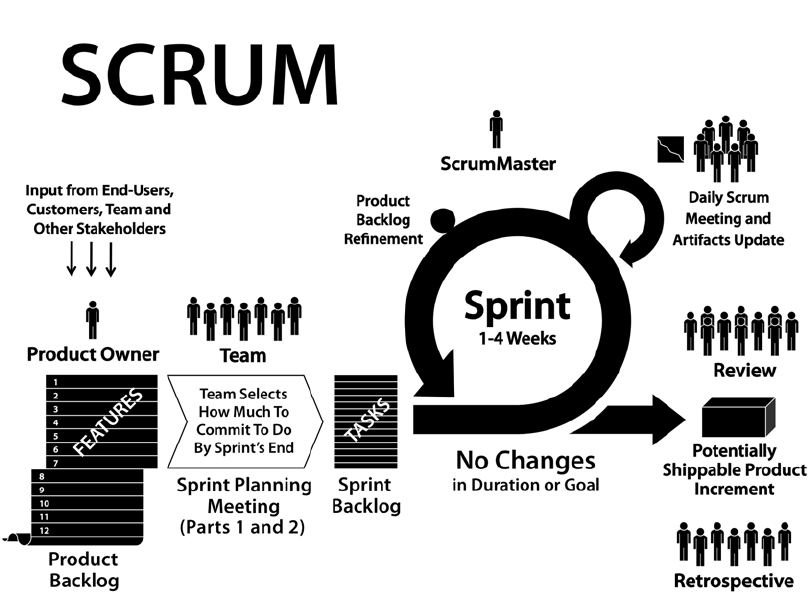
\includegraphics[width=15cm]{figuras/Scrum.png}}
\caption{Metodoloxía Scrum}
\medskip
\small
\centerline{Fonte: \cite{ScrumPrimer}}
\label{ScrumFigure}
\end{figure}

\subsection{Planificación temporal}

Como xa foi explicado, a metodoloxía a empregar neste proxecto trátase da metodoloxía áxil Scrum, na que será posíbel escoller unha tarefa ou serie de tarefas cada vez que se realice un novo \textit{sprint}, e que pretende dar resposta a un nivel grande de incerteza. Ademais, é moi probábel que novas tarefas sexan engadidas á lista de tarefas a medida que o proxecto avanza e vaise dando resposta a certos termos que non resultan claros dende o comezo. Porén, achouse innecesaria a realización dunha planificación temporal ao comezo do proxecto, unha perspectiva enfocada ás metodoloxías pesadas ou clásicas, onde todos os requisitos xa están definidos dende o comezo do proxecto. Deste xeito, enténdese que, aínda seguindo unha estrutura xeral, que será exposta na \gls{EDT} presentada na sección \ref{EDTT}, será posíbel e probábel que xurdan novos requisitos a medida que son cumpridos os requisitos de maior importancia, o que fai realmente complicada a realización dunha planificación temperá con exactitude.\\

Asumindo polo tanto o nivel de incerteza ao que se afronta o proxecto, sobre todo no seu comezo, considérase que non é factíbel a realización dunha planificación temporal extensa, ao non ter coñecemento de todos os requisitos que poderán xurdir a medida que o mesmo avance.\\

Deste xeito, tendo en conta as argumentacións anteriores, conclúese que non paga a pena a realización dun diagrama de Gantt para a realización dunha planificación temporal exhaustiva.

\subsection{Estrutura de detalle do traballo}
\label{EDTT}

Aínda existindo un grande nivel de incerteza e non sendo factíbel a realización dunha planificación temporal exhaustiva, si que resulta posíbel incluso dende o comezo do proxecto, a realización dunha división do traballo a realizar en diferentes módulos. Así, realizarase unha \gls{EDT}, que atendendo ao PMBOK \cite{PMBOK}, outorga unha visión global dende o máis xeral ao máis específico do alcance do proxecto e amosa dun xeito xerárquico o traballo que é preciso realizar para a súa realización. Dita \gls{EDT} está representada na figura \ref{EDTTFigura}.

\begin{figure}
\centerline{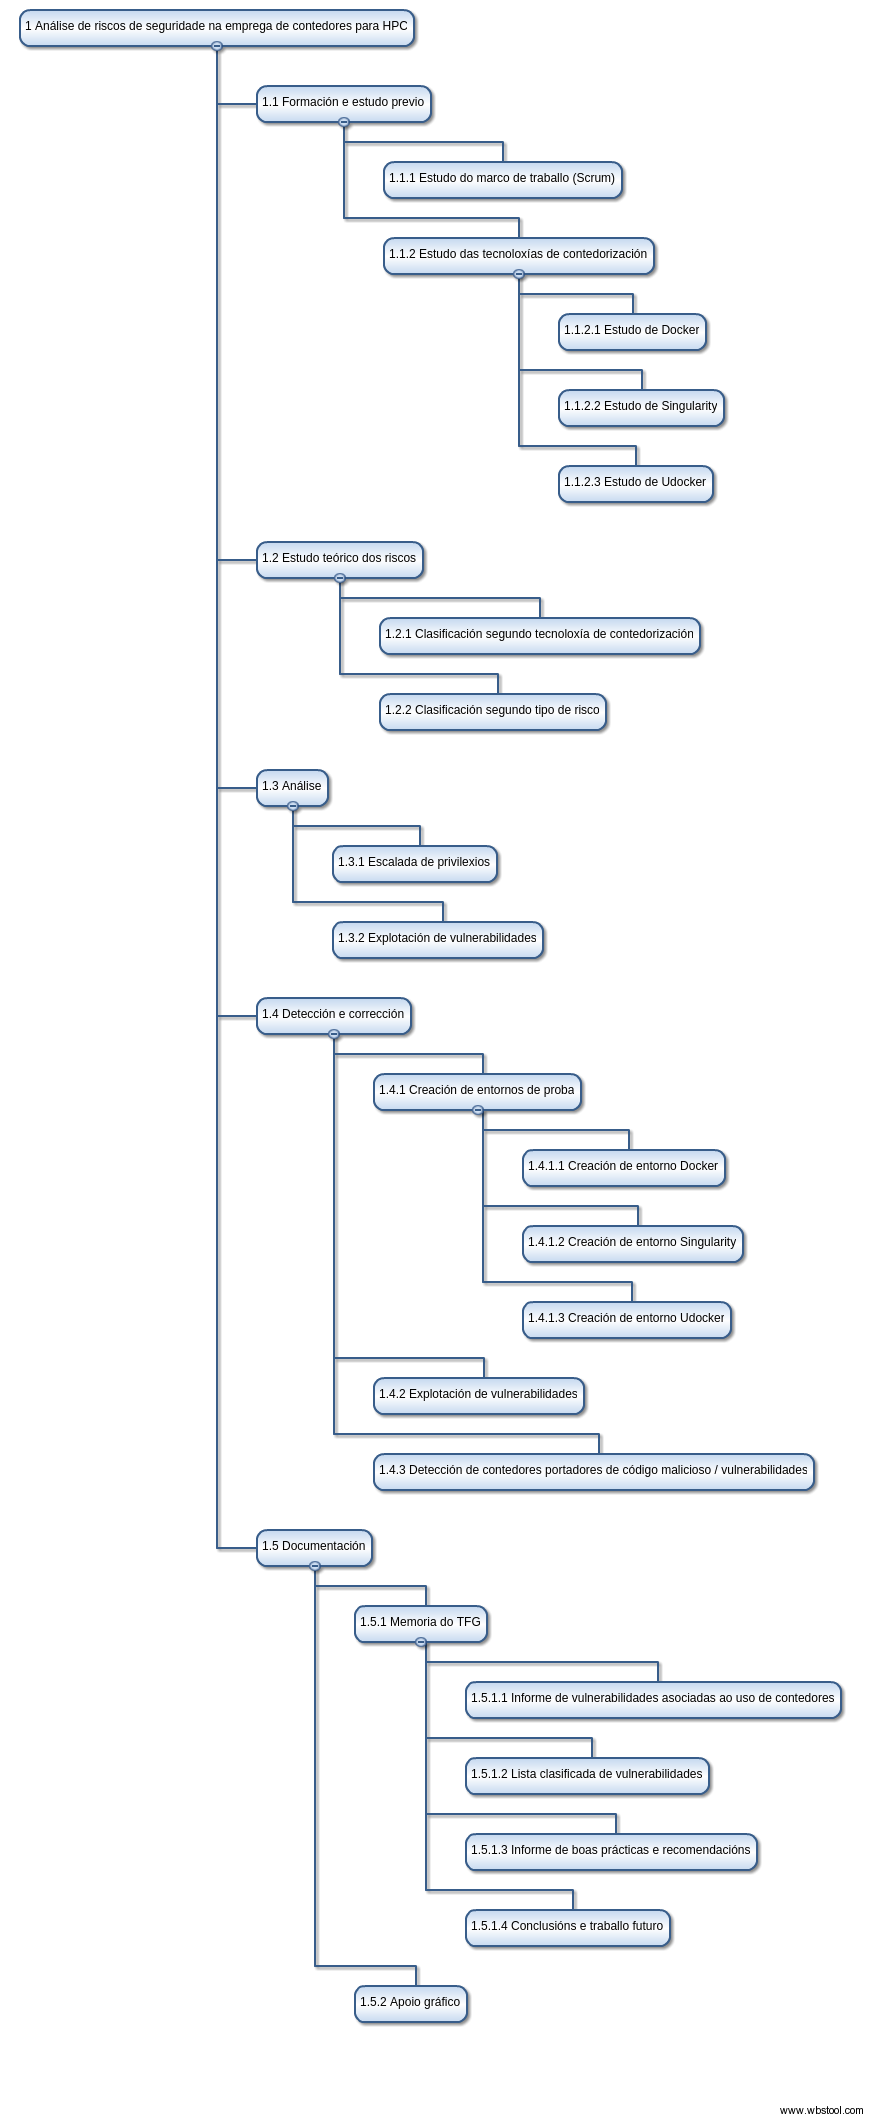
\includegraphics[width=9cm]{figuras/EDTT.png}}
\caption{\gls{EDT} do proxecto}
\label{EDTTFigura}
\end{figure}

\subsection{División temporal xeral das principais fases do proxecto}
\label{divisionTemporalXeral}

Xa foi explicado que resulta complicado realizar unha estruturación temporal detallada do proxecto. Non obstante, contando co detalle de traballo do proxecto, representada na \gls{EDT} da sección \ref{EDTT}, e asumindo as grandes limitacións de tempo ás que se afronta este proxecto, xa que presenta un tempo de desenvolvemento máximo de 412.5 horas, si que resulta posíbel realizar unha división temporal xeneralizada a alto nivel sobre as fases principais do proxecto. O traballo semanal previsto é dunhas 24 horas semanais. O estudo resultante é o seguinte:

\subsubsection{Formación e estudo previo}

\begin{itemize}
    \item \textbf{Duración:} 2 semanas.
    \item \textbf{Descrición:} a pesar de que o autor xa posúe experiencia tratando con tecnoloxías de contedorización, será preciso que revise os seus coñecementos. Tamén cómpre que o autor entenda e interiorice os trazos principais da metodoloxía de traballo, para poder póla en práctica ao longo do proxecto.
\end{itemize}

\subsubsection{Estudo teórico dos riscos}

\begin{itemize}
    \item \textbf{Duración:} 2 semanas.
    \item \textbf{Descrición:} aínda que o autor deste proxecto xa conta con experiencia previa no traballo con tecnoloxías de contedorización, é preciso que adique unha cantidade de tempo razoábel á lectura de artigos referentes á seguridade dos mesmos ou doutras tecnoloxías de virtualización, co fin de identificar os riscos existentes neste eido. A medida que o estudo avance, realizarase unha clasificación, tanto segundo a tecnoloxía como segundo o tipo de risco (rede, explotación de vulnerabilidades, etc.)
    
    É moi probábel que a medida que se investiguen diferentes aspectos relacionados coa seguridade desta tecnoloxía sexa preciso procurar información novamente, sobre temas máis específicos ou facer varias repeticións para asegurar o seu correcto entendemento. Isto quere dicir que é posíbel que esta fase, nun principio introdutoria, esténdase ao longo da totalidade do proxecto.
\end{itemize}

\subsubsection{Análise}

\begin{itemize}
    \item \textbf{Duración:} 4 semanas
    \item \textbf{Descrición:} realizada unha detección dos riscos asociados ás tecnoloxías de contedorización, cómpre realizar unha análise intensiva dos mesmos. Nesta sección realizarase un estudo principalmente teórico, inspirado noutros estudos e artigos científicos xa desenvolvidos pola comunidade. Tamén abarcará o achegamento dun estudo máis empírico mediante probas sobre os entornos de pre-produción e produción para efectuar noutra fase do proxecto.
\end{itemize}

\subsubsection{Detección e corrección}

\begin{itemize}
    \item \textbf{Duración:} 6 semanas.
    \item \textbf{Descrición:} nesta fase crearanse os entornos de proba para poder realizar un estudo empírico das diferentes vulnerabilidades atopadas en etapas anteriores. Inclúe a instalación e despregamento de ferramentas externas para dito estudo, como por exemplo a configuración de ferramentas para a detección de vulnerabilidades en imaxes.
    
    Do mesmo xeito, serán efectuadas diversas probas para evidenciar os riscos aos que se expón un sistema baseado en contedores. Esta fase estará amplamente ligada coa fase de formación e análise, confluíndo probabelmente no tempo, a medida que o factor de incerteza se vai reducindo.
\end{itemize}

\subsubsection{Documentación}

\begin{itemize}
    \item \textbf{Duración:} 3 semanas
    \item \textbf{Descrición:} esta fase supón a redacción da actual memoria, así como a elaboración de todos as figuras e gráficos precisos para a realización de explicacións visuais. Supón á súa vez o contido do traballo, ao non ser un traballo de desenvolvemento software, posto que non existe a penas código (limitado aos \textit{scripts} de configuración ou probas).
    
    É por tanto unha das partes máis cruciais do proxecto, pois é onde deben quedar reflectidos todos os avances feitos. Seguramente tamén teña lugar de xeito paralelo con outras fases, para non esquecer ou perder a información obtida.
\end{itemize}

\section{Presupostos}

Esta sección terá como obxectivo a elaboración dos presupostos do proxecto. Para tal fin, farase unha división entre custos materiais e custos asociados aos recursos humanos. Ademais, tamén debemos diferenciar:

\begin{itemize}
    \item \textbf{Custos directos:} vinculados exclusivamente co desenvolvemento deste proxecto.
    \item \textbf{Custos indirectos:} repartidos entre diferentes proxectos desenvolvidos no mesmo lugar de traballo. Xeralmente son calculados como unha porcentaxe dos custos directos. Un exemplo é o consumo de luz ou auga.
\end{itemize}

\subsection{Custos directos}

\subsubsection{Custos materiais}
\label{custosMateriaisDirectos}

O listado de custos materiais precisos para o desenvolvemento deste proxecto son:

\begin{itemize}
    \item \textbf{Equipo de traballo:} composto por un ordenador de sobremesa, pantalla, teclado e rato. Estímase un valor total duns 1000\euro, e unha vida media duns 6 anos para dito equipo. Tendo en conta a duración deste proxecto, o custo do equipo é de 55.56\euro, tal e como amosan os cálculos da táboa \ref{custoEquipoTraballo}.
    
    \begin{table}[H]
    \centering
    \caption{Custo calculado do equipo de traballo}
    \label{custoEquipoTraballo}
    \begin{tabular}{|c|c|c|c|}
    \hline
    Meses de vida & Meses de uso no proxecto & Custo total & Custo no proxecto \\ \hline
    72 & 4 & 1000\euro & 55.56\euro \\ \hline
    \end{tabular}
    \end{table}
    
    \item \textbf{Material funxíbel:} material físico para a realización do proxecto como bolígrafos, carpetas, cadernos, fotocopias, etc. Estímase nuns 20\euro.
    \item \textbf{Software:} todo o software a empregar ao longo do proxecto será libre ou, ao menos, de balde, polo que non suporá ningún custo no proxecto. Polo tanto, isto limitará a tecnoloxía de Docker á edición \textit{Community Edition} (CE), a cal é gratuíta, quedando descartada a edición \textit{Enterprise Edition} (EE), de pago.
    \item \textbf{Custos computacionais do \gls{FT2}:} no desenvolvemento do proxecto farase uso dos medios computacionais do \gls{CESGA}. Aínda que estes son recursos compartidos, existen medidas que permiten a reserva de recursos limitados, cos que a súa contabilización será moito máis sinxela. O custo aproximado de utilización dos recursos é duns 3 céntimos de euro por procesador por minuto. Tendo en conta as probas que será preciso realizar, estímase a emprega duns 12 procesadores (distribuídos en varias máquinas virtuais), durante unhas 70 horas, polo que os gastos totais asociados a computación ascenderían a 1512\euro.
\end{itemize}

Os custos directos asociados aos materiais do proxecto poden ser consultados na táboa \ref{custosDirectosMateriais}.

\begin{table}[]
\centering
\caption{Custos directos asociados aos materiais}
\label{custosDirectosMateriais}
\begin{tabular}{|c|c|}
\hline
\textbf{Nome} & \textbf{Custo} \\ \hline
Equipo de traballo & 55.56\euro \\ \hline
Material funxíbel & 20\euro \\ \hline
Software & 0\euro \\ \hline
Custos computacionais & 1512\euro \\ \hline \hline
\textbf{TOTAL} & \textbf{1587.56\euro} \\ \hline
\end{tabular}
\end{table}

\subsubsection{Custos de persoal}
\label{custosPersoaisDirectos}

Para realizar o cálculo dos custos asociados aos \gls{RRHH} involucrados no desenvolvemento deste proxecto, cómpre diferenciar os diferentes roles que toman parte no mesmo. Podemos distinguir:

\begin{itemize}
    \item \textbf{Director do proxecto:} rol asumido por ambos os dous titores do proxecto, tendo como labor a supervisión do mesmo e a titorización. Sumaranse as horas de ambos para o cálculo total.
    \item \textbf{Xefe do proxecto:} o seu labor e a redacción da memoria, a corrección da mesma, planificación temporal, análise de riscos, presupostos, etc.
    \item \textbf{Asistente á investigación:} o seu labor consiste na investigación de vulnerabilidades en entornos de contedores para \gls{HPC}, así como en reflectir todos os avances atopados e probas na memoria.
\end{itemize}

Para o cálculo dos salarios empregarase a ferramenta en liña Experteer\footnote{\url{https://www.experteer.es/}} para obter o salario bruto anual e asumirase un custo dun 32\% para o cálculo da Seguridade Social.  A partir desas medidas calcularanse os custos por este proxecto, asumindo un total 14 pagas ao ano e unha xornada laboral 8 horas diarias e 20 días laborábeis ao mes. Os cálculos poden ser observados na táboa \ref{calculoSalarios}.

\begin{table}[H]
\centering
\caption{Cálculo dos salarios dos diferentes roles do proxecto}
\label{calculoSalarios}
\resizebox{\textwidth}{!}{%
\begin{tabular}{|l|c|c|c|c|c|}
\hline
\textbf{Rol} & \textbf{Bruto anual} & \textbf{Seguridade Social} & \textbf{Total anual} & \textbf{Total mensual} & \textbf{Custo/hora} \\ \hline
Director do proxecto & 38000\euro & 12160\euro & 50160\euro & 3583\euro & 22.39\euro \\ \hline
Xefe do proxecto & 32000\euro & 10240\euro & 42240\euro & 3017\euro & 18.86\euro \\ \hline
Asistente á investigación & 17000\euro & 5440\euro & 22440\euro & 1603\euro & 10.01\euro \\ \hline
\end{tabular}
}
\end{table}

Obtidos os diferentes custos por hora, é posíbel deducir os gastos directos asociados aos \gls{RRHH} deste proxecto, que poden ser consultados na táboa \ref{custosDirectosRRHH}.

\begin{table}[H]
\centering
\caption{Custos directos asociados aos \gls{RRHH}}
\label{custosDirectosRRHH}
\begin{tabular}{|l|c|c|c|}
\hline
\textbf{Rol} & \textbf{Custo/hora }& \textbf{Número de horas} & \textbf{Custo total} \\ \hline
Director do proxecto & 22.39\euro & 20 & 447.80\euro \\ \hline
Xefe do proxecto & 18.86\euro & 90 & 1697.40\euro \\ \hline
Asistente á investigación & 10.01\euro & 310 & 3103.10\euro \\ \hline \hline
\textbf{TOTAL} & \multicolumn{2}{l|}{} & \textbf{5248.30\euro} \\ \hline
\end{tabular}
\end{table}

\subsubsection{Custos directos totais}

Obtidos os custos directos materiais (\ref{custosMateriaisDirectos}) e de persoal (\ref{custosPersoaisDirectos}), podemos obter o total dos custos directos, que ascende a un \textbf{total de 6835.86\euro}.

\begin{table}[H]
\centering
\caption{Custos directos totais}
\label{custosDirectosTotais}
\begin{tabular}{|l|c|}
\hline
\textbf{Tipo} & \textbf{Custo asociado} \\ \hline
Material & 1587.56\euro \\ \hline
Persoal & 5248.30\euro \\ \hline \hline
\textbf{TOTAL} & \textbf{6835.86\euro} \\ \hline
\end{tabular}
\end{table}

\subsection{Custos indirectos}

Tendo en conta o marco no que se desenvolve este proxecto, realizado no \gls{CESGA} e no Departamento de Electrónica e Computación da Universidade de Santiago de Compostela, decidiuse seguir as políticas de custos en I+D da Universidade \cite{xestionEconomicaUSC}, a cal indica que se deben calcular tomando como referencia un 20\% dos custos directos totais. Deste xeito, os custos indirectos ascenden a un \textbf{total de 1307.12\euro}.

\subsection{Custos totais}

Os custos totais calcúlanse como a suma dos custos directos e indirectos. Os custos totais deste proxecto ascenden a un \textbf{total de 8143.03\euro}.

\begin{table}[H]
\centering
\caption{Custos totais}
\label{custosTotais}
\begin{tabular}{|l|c|}
\hline
\textbf{Tipo} & \textbf{Custo asociado} \\ \hline
Directo & 6835.86\euro \\ \hline
Indirecto & 1307.12\euro \\ \hline \hline
\textbf{TOTAL} & \textbf{8143.03\euro} \\ \hline
\end{tabular}
\end{table}

\section{Alcance do proxecto}

\subsection{Descrición do alcance}

O presente proxecto ten como finalidade o estudo de vulnerabilidades na emprega de contedores para \gls{HPC}. Tal cometido entenderase rematado coa obtención dunha lista clasificada de vulnerabilidades, un estudo das mesmas, unha documentación de boas prácticas e recomendacións así como unha serie de conclusións e traballo futuro para a posíbel continuidade do proxecto.

\subsection{Entregábeis do proxecto}

Os entregábeis deste proxecto consisten nesta propia memoria, con todos os estudos xa realizados e as conclusións obtidas, así como todos as figuras realizadas para a súa explicación visual e os \textit{scripts} precisos para a reproducibilidade das probas.

\subsection{Exclusións do proxecto}

Quedarán descartadas aquelas tarefas que pola súa complexidade incrementen notabelmente o tempo planificado para a execución da división temporal xeral das principais fases do proxecto, establecidas na sección \ref{divisionTemporalXeral}. Non debemos esquecer que este se trata dun proxecto asociado a un Traballo de Fin de Grao, polo que a súa limitación temporal é moi forte e debe ser respectada.

\subsection{Supostos do proxecto}

Asúmese que dende o comezo do proxecto o autor deste proxecto contará con acceso a todos os medios necesarios para realizar as probas que considere precisas (acceso aos entornos de pre-produción e produción).

\subsection{Restricións do proxecto}

\begin{itemize}
    \item Duración máxima do proxecto: 4 meses.
    \item Data máxima de entrega da memoria: 2 de xullo de 2018.
\end{itemize}
